\documentclass{article}
\usepackage{graphicx} % Required for inserting images
\usepackage[utf8]{inputenc}
\usepackage{polski}
\usepackage[dvipsnames]{xcolor}
\usepackage{indentfirst}
\usepackage{multicol}
\usepackage{geometry}
\usepackage{titlesec}
\usepackage[colorlinks=true, linkcolor=gray, urlcolor=blue, citecolor=green]{hyperref}
\usepackage{makecell}
\usepackage{float}
\usepackage[polish]{babel}
\usepackage[T1]{fontenc}
\usepackage[justification=centering]{caption}
\usepackage[utf8]{inputenc} 
\usepackage{subfig}
\usepackage{changepage}


\usepackage{mwe} % for 'example-image'
\usepackage{newfloat}
\DeclareFloatingEnvironment{graph}
\addto\captionspolish{%
  \renewcommand{\graphname}{Wykres}%
  \renewcommand{\figurename}{Zdjęcie}%
  \renewcommand{\tablename}{Tabela}%
}


\begin{document}

\begin{titlepage}
    \begin{center}
        \vspace*{1cm}
            
        \Huge
        \textbf{Sprawozdanie z laboratorium 2}
            
        \vspace{0.5cm}
        \LARGE
        Podstawy PLC (Siemens) 
            
        \vspace{1.5cm}
            
        \textbf{Łukasz Janusz\\Marek Generowicz}

        \normalsize      
        \textcolor{gray}{03.04.2025}
        \vfill
        \begin{figure}[hb]
            \centering
            
\includegraphics[width=0.5\textwidth]{media/Logo_AGH.jpg}
        \end{figure}   
    \end{center}
\end{titlepage}

\newpage
\section{Wstęp}
Na zajęciach należało zapoznać się z podstawami programowania sterowników PLC, na tych ćwiczeniach do dyspozycji posiadaliśmy  sterownik \textit{S7 - 1200} marki Siemens, który jest przedstawiony na zdjęciu \ref{fig:zdj21}. Całe stanowisk składało się z poniższych części:

\begin{itemize}
    \item \textbf{Pompy} 
    \item \textbf{Zbiornika} 
    \item \textbf{Elektrozaworów solenoidowych}
    \item \textbf{Zaworów ręcznych}  
\end{itemize}

Za pomocą PLC możliwe było sterowane były elektrozawory, dzięki którym można było kontrolować ciśnienie w rurociągach co poprzez presostat załączenie pompy pozwalającej na przelewanie cieczy do zbiornika. Na zdjęciu \ref{fig:zdj37} przedstawione jest całe stanowisko, które było wykorzystywane podczas ćwiczeń.

Ponadto w układzie możliwe były pomiary przepływu i ciśnienia oraz poziomu i temperatury cieczy w zbiorniku.

\begin{figure}[H]
    \centering
        % Pod figura 1
        \subfloat[PLC obsługujący elektrozawory (zdjęcie z konspektu)]{    
            \centering
            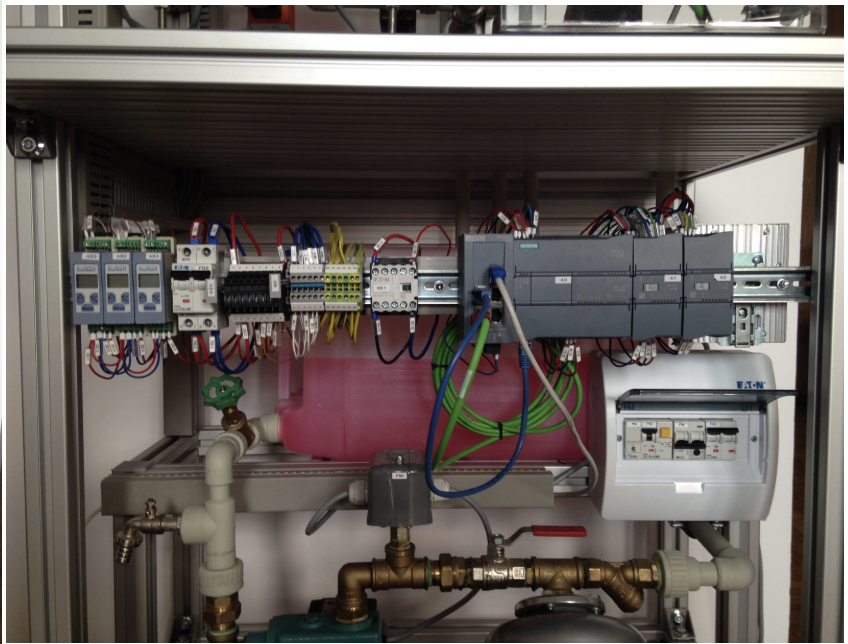
\includegraphics[width=0.5\textwidth]{media/0_2_PLC.png}
            \label{fig:zdj21}}
        % Pod figura 1
        \subfloat[Całe stanowisko (zdjęcie z konspektu)]{
            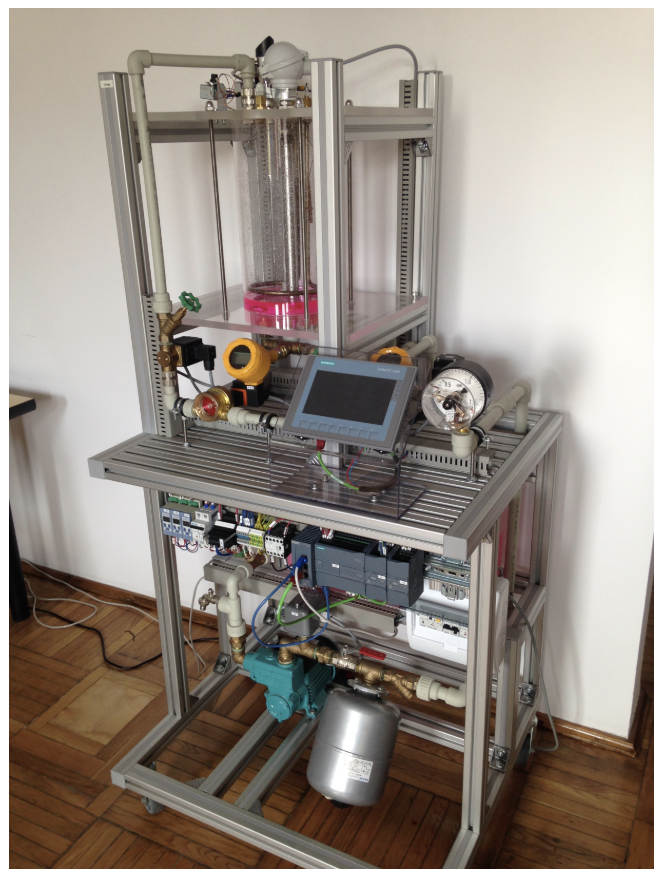
\includegraphics[width=0.5\textwidth]{media/0_1_Całe_stanowisko.png}
            \label{fig:zdj37}}
    \caption{Konfiguracja kanałów modułu}
    \label{fig:main0}
\end{figure}


\section{Konfiguracja sterownika}
Na początku ćwiczenia należało skonfigurować sterownik PLC w aplikacji \textit{TIA Portal V19} aby można było odczytać wejścia analogowe oraz zapisać wyjścia analogowe. W tym celu należało na początku należało dodać jednostkę centralną, a następnie dodać dwa moduły wejść/wyjść analogowych, które w kolejnych krokach pozwolą nam na obsługę elektrozaworów.

Po poprawnej konfiguracji wirtualny schemat układu z PLC wyglądał tak jak na zdjęciu \ref{fig:zdj1}.
\begin{figure}[H]
    \centering
    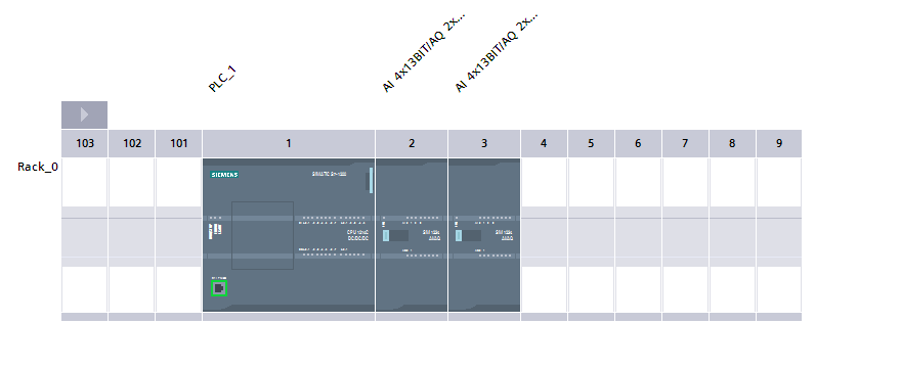
\includegraphics[width=0.5\textwidth]{media/1_1_Dodanie_modułu.png}
    \caption{Wirtualny układ z PLC}
    \label{fig:zdj1}
\end{figure}

Następnie należało ustawić poprawny adres IP, aby można było połączyć się z PLC. W tym celu należało kliknąć prawym przyciskiem myszy na jednostkę centralną i wybrać opcję \textit{Properties}, a następnie w zakładce \textit{PROFINET Interface} ustawić poprawny adres IP. Na zdjęciu \ref{fig:zdj2} przedstawione są ustawienia sieciowe PLC.
\begin{figure}[H]
    \centering
    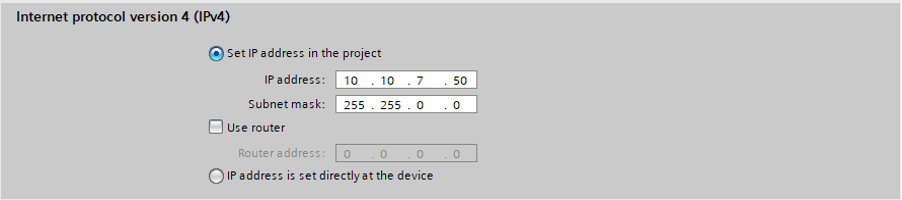
\includegraphics[width=0.5\textwidth]{media/1_2_Ustawienia_sieciowe_PLC.png}
    \caption{Ustawienia sieciowe PLC}
    \label{fig:zdj2}
\end{figure}

Po poprawnym wykonaniu można było połączyć się z PLC. Poprawne skonfigurowanie i wejście w tryb Online skutkowało, że Interface w aplikacji wyglądał tak jak na zdjęciu \ref{fig:zdj3}. Dzięki temu można było przejść do kolejnych kroków ćwiczenia.
\begin{figure}[H]
    \centering
    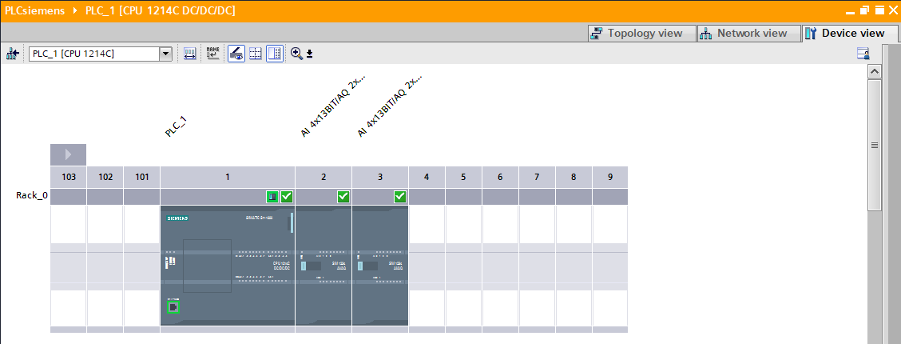
\includegraphics[width=0.5\textwidth]{media/1_3_PLC_Online.png}
    \caption{Poprawne połączenie z PLC}
    \label{fig:zdj3}
\end{figure}


\newpage
\section{Odczyt i zapis zmiennych procesowych}
Po poprawnym połączeniu z PLC należało skonfigurować moduły analogowe zgodnie z schematem stanowiska. Wszystkie kanały w module 1 oraz pierwszy kanał w module 2 należało skonfigurować zgodnie tak jak na zdjęciu \ref{fig:zdj4} natomiast pozostałe kanały w module 2 należało skonfigurować tak jak na zdjęciu \ref{fig:zdj5}, dzięki czemu moduły które nie będą wykorzystywane nie będą zgłaszać błędów. Ważne było również aby wszystkie z wejść były wejściami prądowymi w zakresie od 4 do 20 mA.
\begin{figure}[H]
    \centering
    \includegraphics[width=0.5\textwidth]{media/2_1_Ustawienia_wejść_IO.png}
    \caption{Przykład konfiguracji aktywnych kanałów wejść}
    \label{fig:zdj4}
\end{figure}

\begin{figure}[H]
    \centering
    \includegraphics[width=0.5\textwidth]{media/2_2_Ustawienia_wejść_IO_OFF.png}
    \caption{Przykład konfiguracji kanałów wejść nieaktywnych}
    \label{fig:zdj5}
\end{figure}

Natomiast w obu modułach wszystkie kanały wyjść miały wyglądać tak jak na zdjęciu \ref{fig:zdj6}. Ważne aby ustawić je jako kanały napięciowe.
\begin{figure}[H]
    \centering
    \includegraphics[width=0.5\textwidth]{media/2_3_Ustawienia_wyjść.png}
    \caption{Przykład konfiguracji kanałów wyjść}
    \label{fig:zdj6}
\end{figure}
\newpage
Po skonfigurowaniu wejść i wyjść należało w każdym z modułów opisać tagi wejść i wyjść zgodnie z opisem w dokumentacji elektrycznej stanowiska. Zdjęcia \ref{fig:main2} przedstawiają jak powinny być przypisane tagi w odpowiednich modułach.
\begin{figure}[H]
    \centering
        % Pod figura 1
        \subfloat[Tagi wejścia i wyjścia dla modułu 1]{    
            \centering
            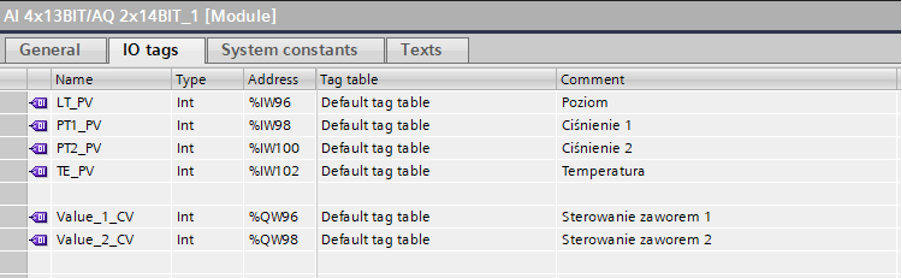
\includegraphics[width=0.5\textwidth]{media/2_4_Tagi_moduł_1.png}
            \label{fig:zdj7}}
        % Pod figura 1
        \subfloat[Tagi wejścia i wyjścia dla modułu 2]{
            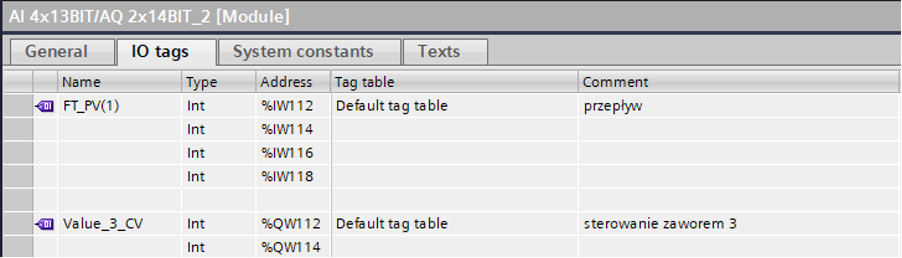
\includegraphics[width=0.5\textwidth]{media/2_5_Tagi_moduł_2.png}
            \label{fig:zdj8}}
    \caption{Konfiguracja kanałów modułu}
    \label{fig:main2}
\end{figure}

Po poprawnym skonfigurowaniu obu modułów należało przesłać ustawienia do sterownika, a następnie stworzyć \textit{Watch table}, która umożliwi nam odczyt wartości tagów. Dzięki temu po przejściu w tryb online nie dość że można było odczytywać parametry takie jak poziom cieczy w zbiorniku, ciśnienia, temperature cieczy w zbiorniku czy przepływ. 

Warto zauważyć że największa wartość jaką możemy otrzymać wynosi 32 767, wynika to z tego że w PLC na każde z wyjść i wejść przypadają 4 miejsca w któ®ych możemy wpisać zmienną w systemie szesnastkowym ($2^{4^4} = 2^{16} = 65536$ ale musimy podzielić to na pół z czego otrzymujemy zakres od 0 do 27648).

Również warta uwagi jest wartość przy przepływie, które wynikają z tego wartości zwracane przez czujnik były poza zakresem, ponieważ czujnik ten powinien być używany do większego przepływu.
\begin{figure}[H]
    \centering
    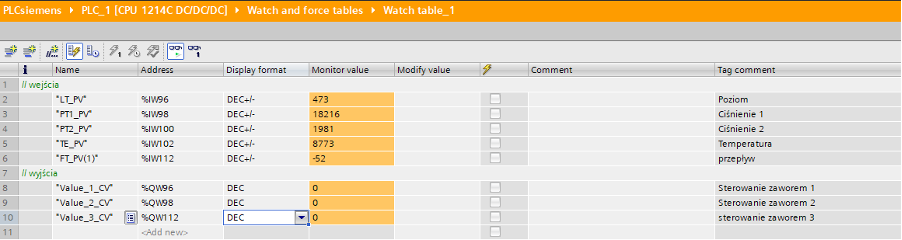
\includegraphics[width=0.5\textwidth]{media/2_6_Watch_tab_Online.png}
    \caption{Podstawowa \textit{Watch Table}}
    \label{fig:zdj9}
\end{figure}

Dodatkowo można było kontrolować zawory, 1 i 2 do zwiększania poziomu cieczy w zbiorniku a 3 do zmniejszania poziomu. 

\newpage
\section{Skalowanie zmiennych procesowych}
W ostatnim zadaniu należało stworzyć funkcję, która będzie skalować zmienne procesowe. Jednak przed przystąpieniem do tworzenia funkcji należało najpierw dodać dodatkowe parametry do PLC tags (tablica została automatycznie uzupełniona po stworzeniu tagów konkretnych modułów), które miały za zadanie odpowiadać wartościom przeskalowanym. Ostateczna tabela PLC tags powinna wyglądać tak jak na zdjęciu \ref{fig:zdj10}

\begin{figure}[H]
    \centering
    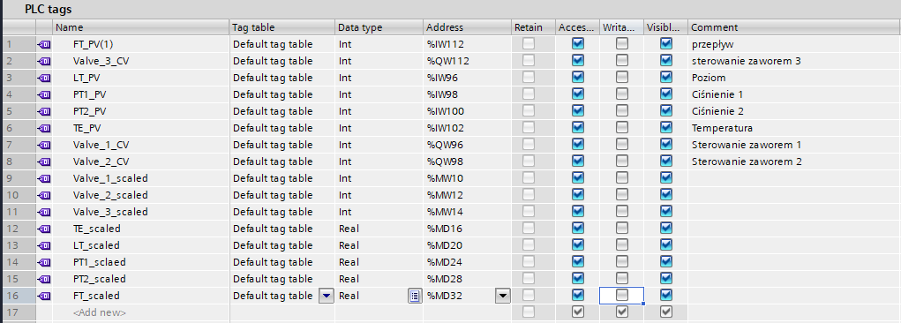
\includegraphics[width=0.5\textwidth]{media/3_1_PLC_tags_scaled.png}
    \caption{Tagi PLC z dodanymi zmiennymi przeskalowanymi}
    \label{fig:zdj10}
\end{figure}


Po stworzeniu wszystkich potrzebnych tagów należało stworzyć funkcję, która będzie odpowiedzialna za przeskalowanie zmiennych procesowych. W tym celu niezbędne było utworzenie zmiennej pomocniczej \textit{temp}, jednak nie trzeba było tworzyć jej dla każdej drabinki osobno z racji że w \textit{TIA Portal} kody wykonują się sekwencyjnie.

\vspace{1em}
Zdjęcie \ref{fig:zdj13} przedstawia jak powinny wyglądać drabinki dla zmiennych wyjściowych. Warto zauważyć że w tym przypadku należało przeskalować zmienną z zakresu od 0 do 100 (odpowiadającemu zakresowi procentowemu) do zakresu od 0 do 27648 aby otrzymać zmienną wyjściową. 


\begin{figure}[H]
    \centering
    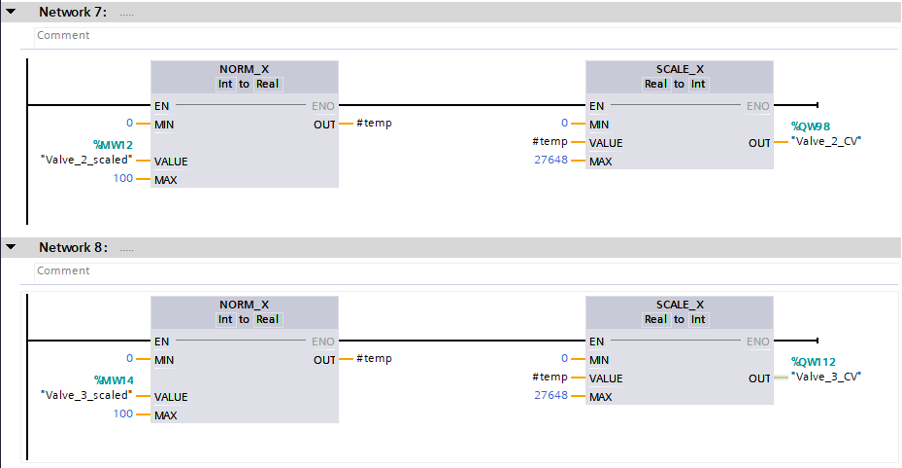
\includegraphics[width=0.5\textwidth]{media/3_2_3_PLC_logika_hej.png}
    \caption{Przeskalowywanie zmiennych wyjściowych}
    \label{fig:zdj13}
\end{figure}

\newpage
Dla każdego z tagów wejścia należało analogiczne funkcje, jednak te miały za zadanie przeskalowywać zmienną z zakresu od 0 do 27648 do zakresu od 0 do 100. Funkcje te przedstawione są na zdjęciach \ref{fig:main420}.
\begin{figure}[H]
    \centering
        % Pod figura 1
        \subfloat[Przeskalowywanie zmiennych poziomu i ciśnienia]{    
            \centering
            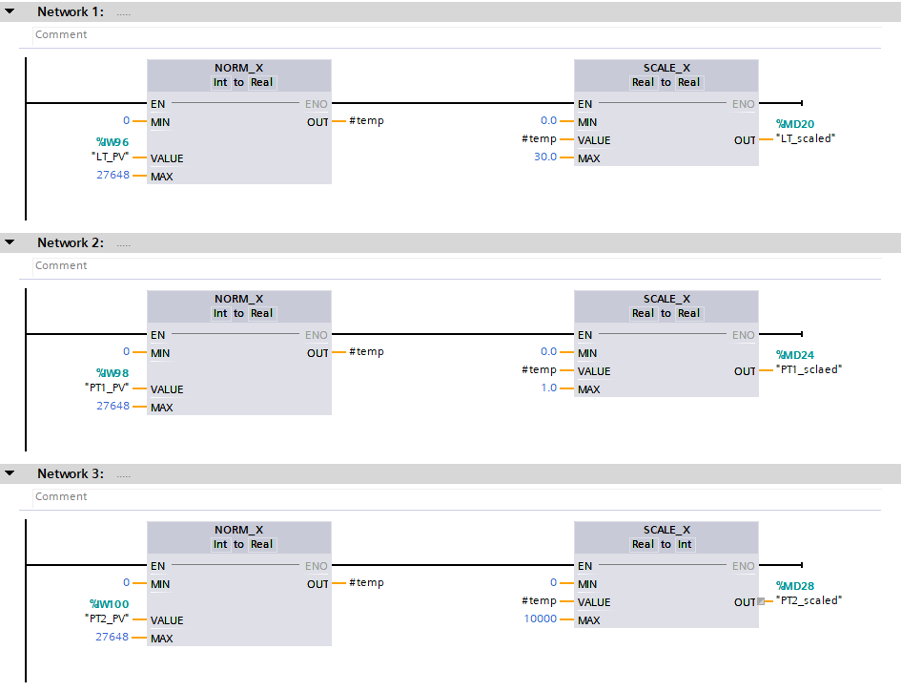
\includegraphics[width=0.5\textwidth]{media/3_2_1_PLC_logika_hej.png}
            \label{fig:zdj11}}
        % Pod figura 1
        \subfloat[Przeskalowywanie zmiennych temperatury i przepływu]{
            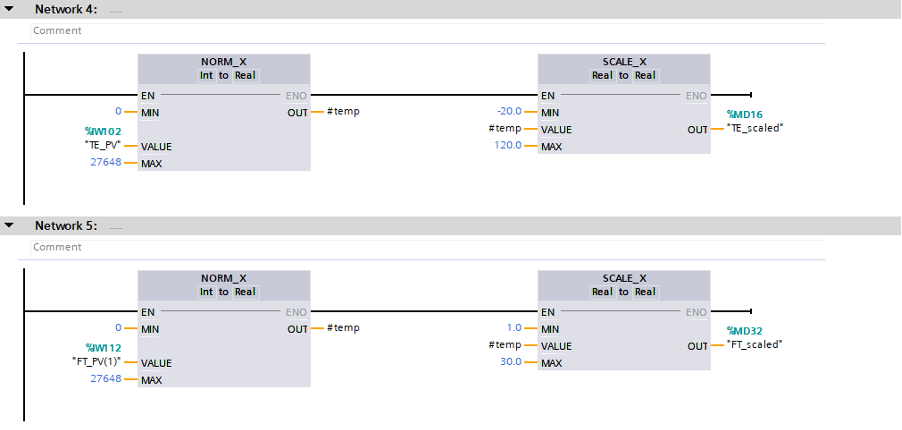
\includegraphics[width=0.5\textwidth]{media/3_2_2_PLC_logika_hej.png}
            \label{fig:zdj12}}
    \caption{Przeskalowywanie zmiennych wejściowych}
    \label{fig:main420}
\end{figure}


Po poprawnym stworzeniu funkcji należało przesłać zmiany na PLC, a następnie przejść w tryb online. Dzięki temu można było odczytać przeskalowane zmienne procesowe oraz ich oryginalne wartości, które były widoczne w \textit{Watch table}. Na zdjęciu \ref{fig:zdj14} przedstawione są wartości z załączonymi pompami 1 (otwartą w 100\%) oraz 2 (otwartą w 75\%), natomiast pompa 3 jest kompletnie zamknięta.
\begin{figure}[H]
    \centering
    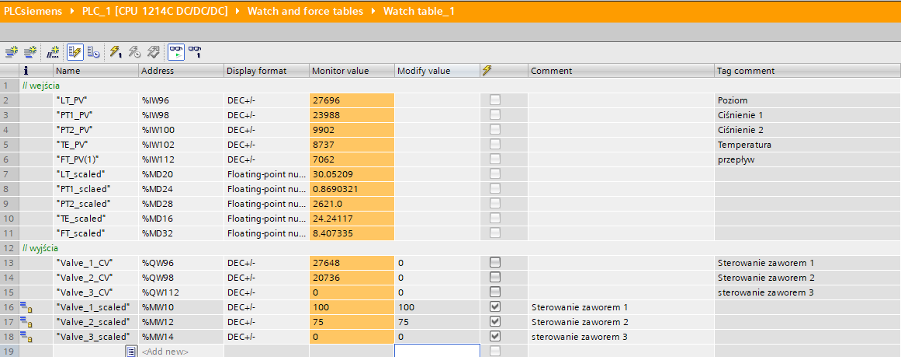
\includegraphics[width=0.5\textwidth]{media/3_3_Watch_table_online.png}
    \caption{Watch table z przeskalowanymi zmiennymi}
    \label{fig:zdj14}
\end{figure}

\newpage
\section{Podsumowanie}
Podczas drugiego laboratorium z podstaw programowania sterowników PLC studenci zapoznali się z konfiguracją oraz obsługą sterownika Siemens S7-1200 w środowisku TIA Portal V19. Głównym celem ćwiczenia było stworzenie kompletnego układu sterowania procesem przemysłowym z wykorzystaniem sygnałów analogowych i cyfrowych.

W ramach zajęć przeprowadzono:
\begin{itemize}
    \item Konfigurację sprzętową sterownika i modułów wejść/wyjść analogowych,
    \item Ustawienie adresów IP oraz konfigurację kanałów pomiarowych w zakresie 4–20 mA dla wejść i 0–10 V dla wyjść,
    \item Nadanie tagów zmiennym procesowym zgodnie z dokumentacją techniczną stanowiska,
    \item Stworzenie tabeli monitorującej Watch Table umożliwiającej bieżący podgląd parametrów procesowych,
    \item 
    Zaimplementowanie funkcji skalujących, przekształcających wartości analogowe do formatu procentowego i odwrotnie, zgodnie z zakresem przetworników (0–27648 → 0–100\%).
\end{itemize}

Zrealizowane działania umożliwiły sterowanie poziomem cieczy w zbiorniku za pomocą elektrozaworów, a także odczyt parametrów takich jak temperatura, ciśnienie, przepływ i poziom. Dzięki zastosowaniu skalowania zmiennych, wartości pomiarowe mogły być wygodnie analizowane i wykorzystywane w logice sterującej. Zajęcia zakończyły się powodzeniem i stanowiły praktyczne wprowadzenie do projektowania systemów automatyki z użyciem TIA Portal i PLC Siemens.
\end{document}
